\subsection{Display > Full Screen}
\label{subsection:fullscreen}

\index{plein �cran}
\par
Cette fonction permet d'afficher la fen�tre principale de \emph{CloudCompare} en plein �cran. Dans
ce mode, la totalit� de l'�cran est occup� par l'application. La barre de titre de \emph{CloudCompare}
ainsi que la barre de tache de Windows ne sont plus accessibles, ce qui am�liore le confort visuel
mais emp�che les manipulations habituelles sur les fen�tres (d�placement, r�duction, changement
de fen�tre active, ...).
\par
Pour repasser en affichage normal, il suffit de cliquer une nouvelle fois sur la commande \emph{Full screen},
ou d'utiliser la touche de raccourci associ�e (F11).\\
\par
Note : il est tout de m�me possible de changer de fen�tre active, m�me en affichage plein �cran,
en maintenant la touche ALT enfonc�e, puis en pressant la touche TAB de mani�re � faire d�filer le s�lecteur
(cf. figure \ref{fig:altTab}) jusqu'� l'application souhait�e. Lorsque la touche ALT est relach�e, Windows active
la fen�tre de l'application ainsi s�lectionn�e. Cette commande est utilisable pour toute application.\\

\begin{figure}[!htb]
\begin{center}
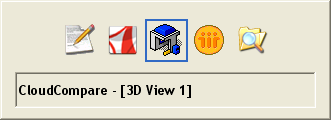
\includegraphics[width=0.5\textwidth]{Partie3_Fonctions/altTab.png}
\caption{\label{fig:altTab}S�lecteur d'application sous Windows}
\end{center}
\end{figure}

\par
\textcolor[rgb]{1.00,0.00,0.00}{Raccourci clavier : F11}
